% !TeX encoding = UTF-8
\documentclass{beamer}
\usepackage{tikz}
\usepackage[utf8]{inputenc}
\usepackage[spanish]{babel}
\usetheme{Hannover}
\usecolortheme{crane}
\usepackage{graphicx}
\usepackage{smartdiagram}
\usepackage{qtree}
\usepackage{listings}
\lstset{language=Java,
                basicstyle=\footnotesize\ttfamily,
                keywordstyle=\footnotesize\color{blue}\ttfamily,
}

\usepackage{graphicx}
\usebackgroundtemplate%
{%
    
\includegraphics[width=\paperwidth]{Images/fondo.png}%
}

\definecolor{celeste}{HTML}{5E91AA}
\definecolor{azul}{HTML}{163F54}

\setbeamercolor{head1}{fg=celeste}
\setbeamercolor{title}{fg=celeste}
\setbeamercolor{subtitle}{fg=celeste}
\setbeamercolor{frametitle}{fg=celeste}
\setbeamercolor{structure}{fg=azul}
\setbeamercolor{normal text}{fg=azul}


\title{Java y su ecosistema}
\author{Víctor Orozco}
\institute{GuateJUG}
\date{\today}

\begin{document}

\frame{\titlepage}

\section{Intro}

\begin{frame}{Víctor Orozco}
    \begin{columns}[T] % contents are top vertically aligned
        \begin{column}[T]{5cm} % each column can also be its own environment
            \begin{itemize}
                \item Developer (JVM/Open Source Advocate)
                \item JUG Leader
                \item Consultor independiente
                \item Profesor universitario
                \item \href{https://twitter.com/tuxtor}{@tuxtor}
                \item \href{http://vorozco.com}{The J*} 
            \end{itemize}
        \end{column}
        \begin{column}[T]{5cm} % alternative top-align that's better for graphics
            \begin{figure}
                \centering
                
\includegraphics[width=0.6\linewidth]{Images/logos}
            \end{figure}
            
        \end{column}
    \end{columns}
\end{frame}

\begin{frame}{Java}
	\begin{figure}
		\centering
		
\includegraphics[width=0.5\linewidth]{Images/chaos}
	\end{figure}
\end{frame}


\section{¿Porque Java?}
\begin{frame}
	\huge ¿Porque Java?
\end{frame}

\begin{frame}
	JAVA IS DEAD
\begin{figure}
	\centering
	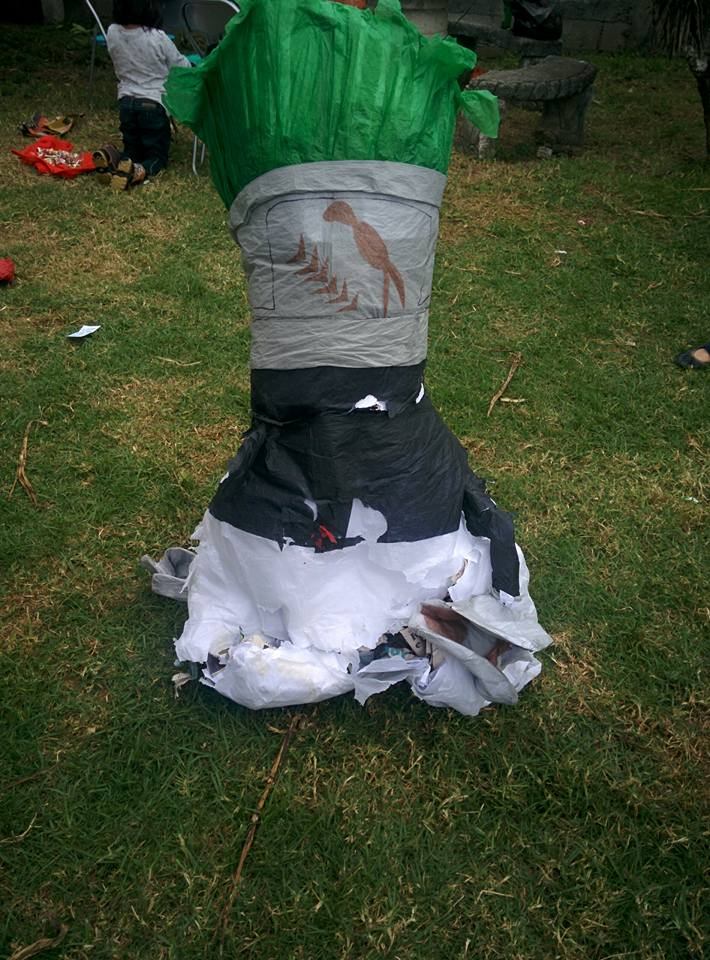
\includegraphics[width=0.5\linewidth]{Images/dukedead.jpg}
\end{figure}
\end{frame}

\begin{frame}
	\begin{figure}
		\centering
		
\includegraphics[width=0.5\linewidth]{Images/javadead}
	\end{figure}
\end{frame}

\begin{frame}
	\begin{figure}
		\centering
		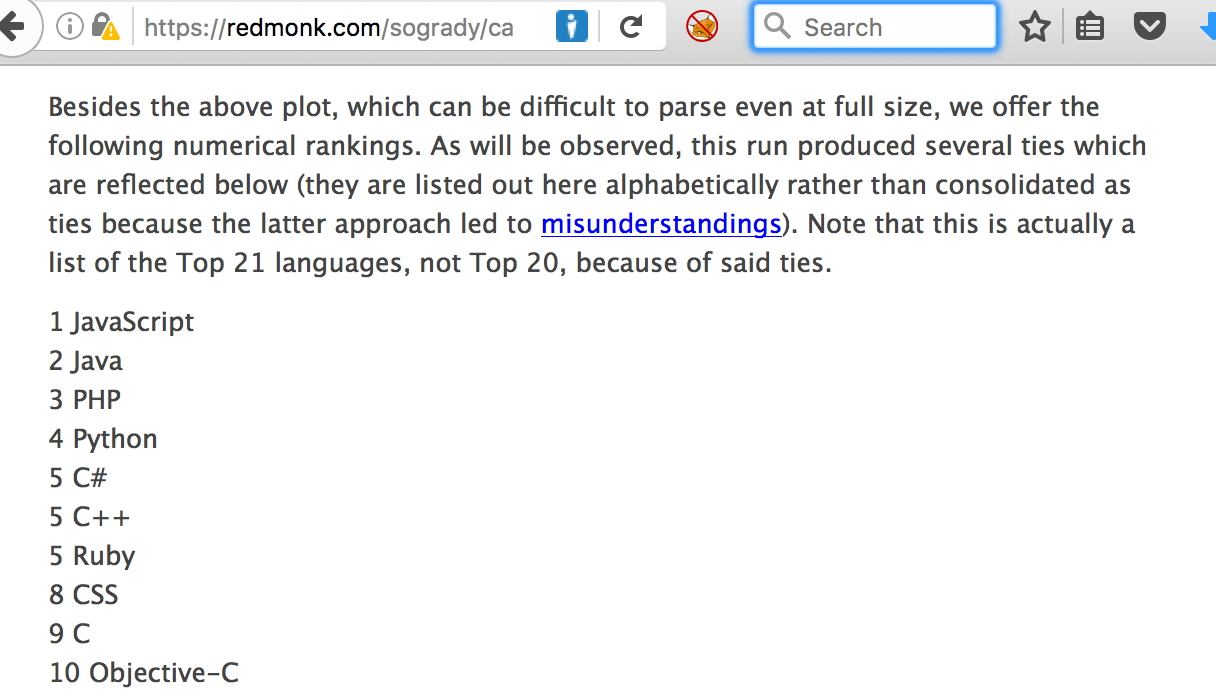
\includegraphics[width=0.9\linewidth]{Images/redmonk}
	\end{figure}
\end{frame}

\begin{frame}
	\begin{figure}
		\centering
		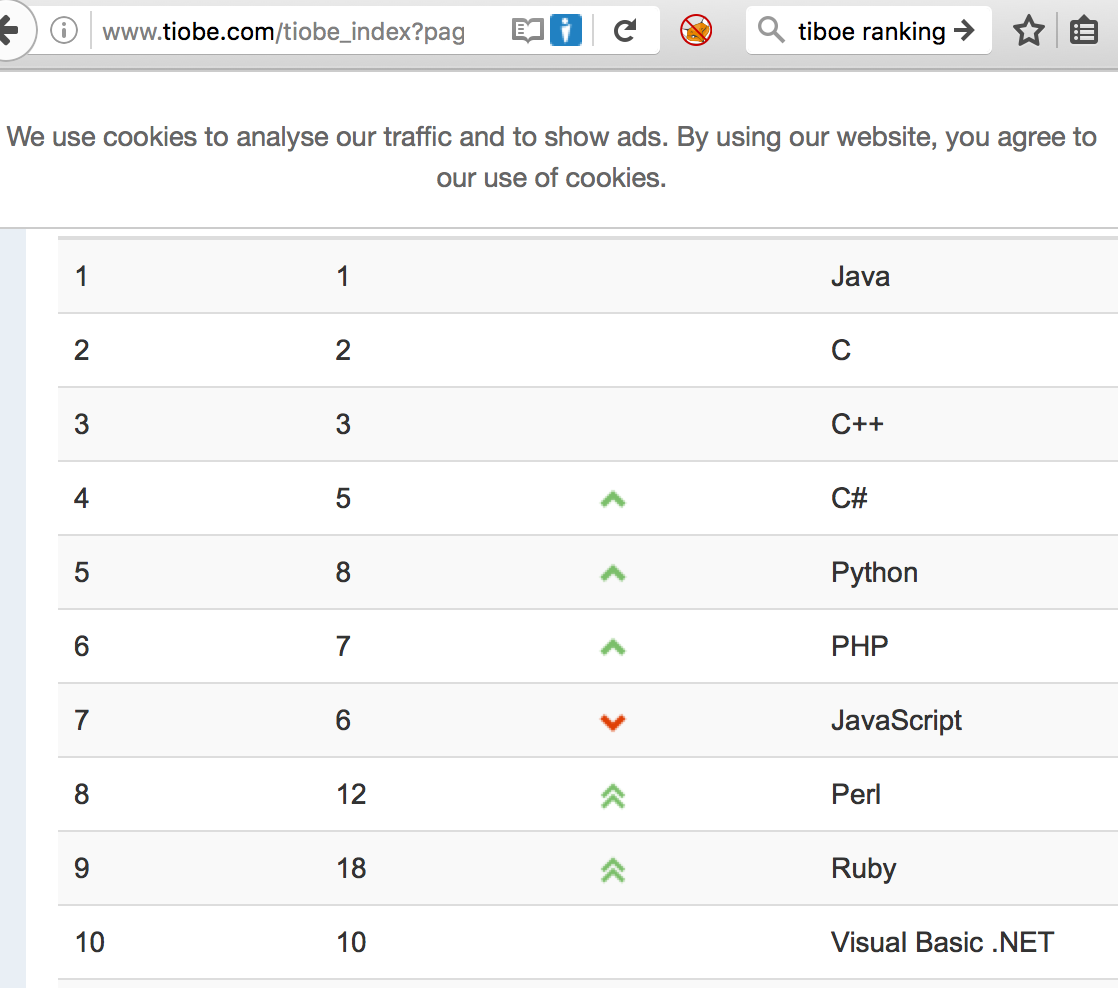
\includegraphics[width=0.9\linewidth]{Images/tiboe}
	\end{figure}
\end{frame}

\section{Java}
\begin{frame}
	\huge ¿Que es Java?
\end{frame}

\begin{frame}{Lenguaje}
	\begin{figure}
		\centering
		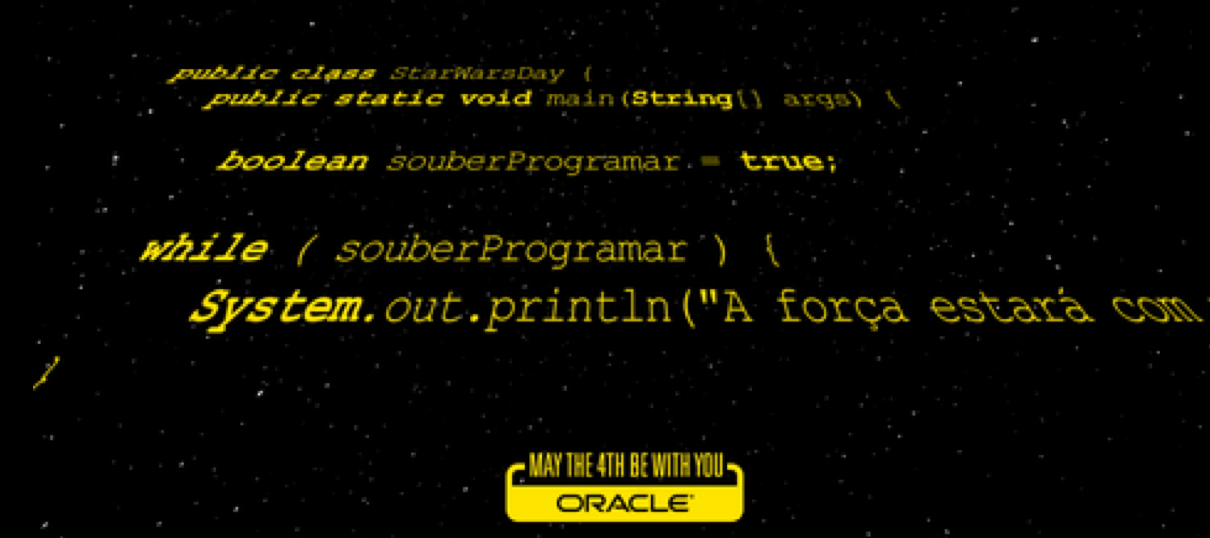
\includegraphics[width=0.9\linewidth]{Images/javalang}
	\end{figure}
\end{frame}

\begin{frame}{Maquina virtual}
	\begin{figure}
		\centering
		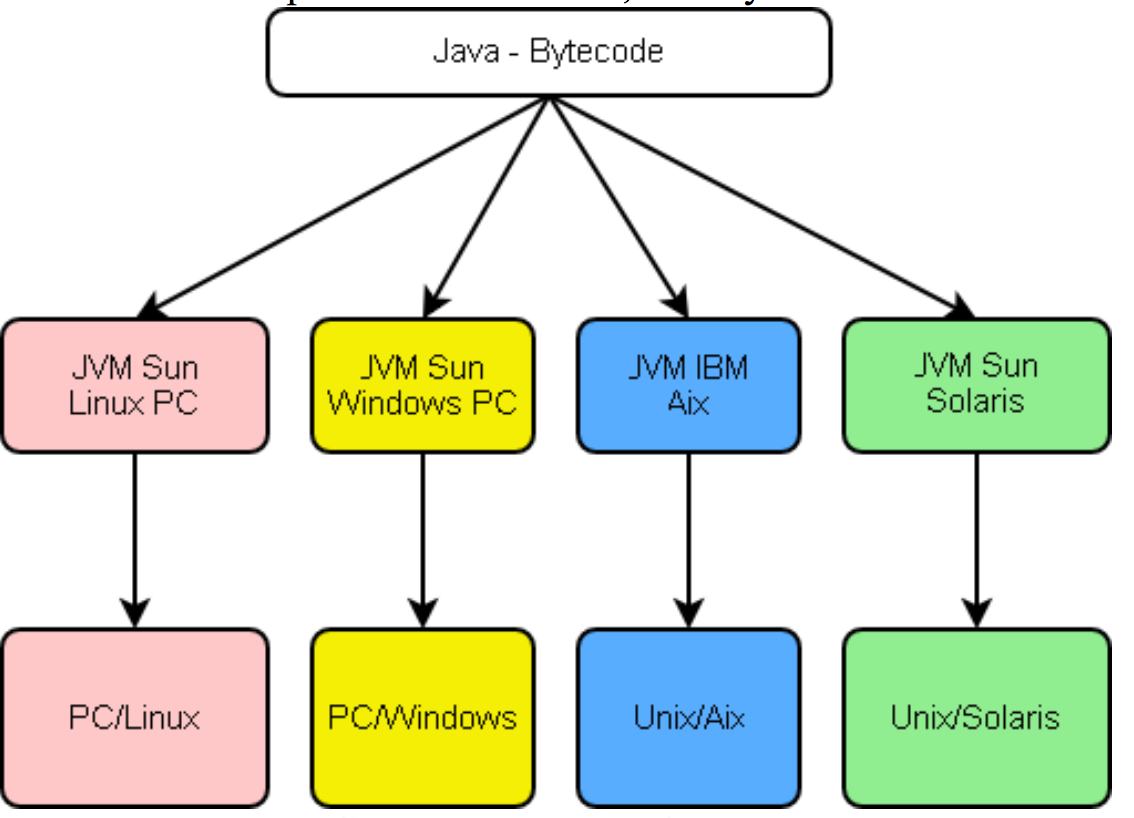
\includegraphics[width=0.9\linewidth]{Images/jvm}
	\end{figure}
\end{frame}

\begin{frame}{Muchas plataformas}
	\begin{figure}
		\centering
		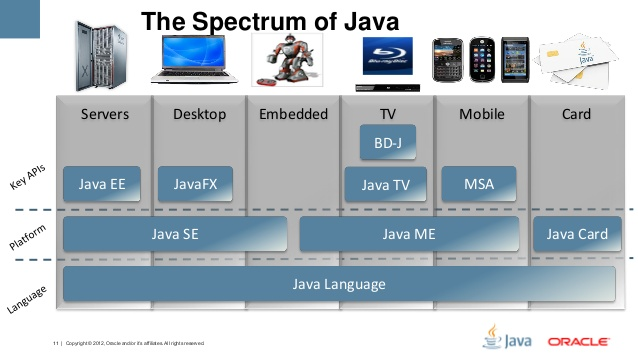
\includegraphics[width=0.9\linewidth]{Images/spectrum}
	\end{figure}
\end{frame}

\section{Java}
\begin{frame}
	\huge ¿Como programar en Java?
\end{frame}

\begin{frame}{Como programar en Java}
	\begin{itemize}
		\item Lenguaje
		\item Objetivo
		\item Maquina
		\item Framework
		\item Herramientas
	\end{itemize}
\end{frame}

\begin{frame}{Lenguaje}
	\begin{figure}
		\centering
		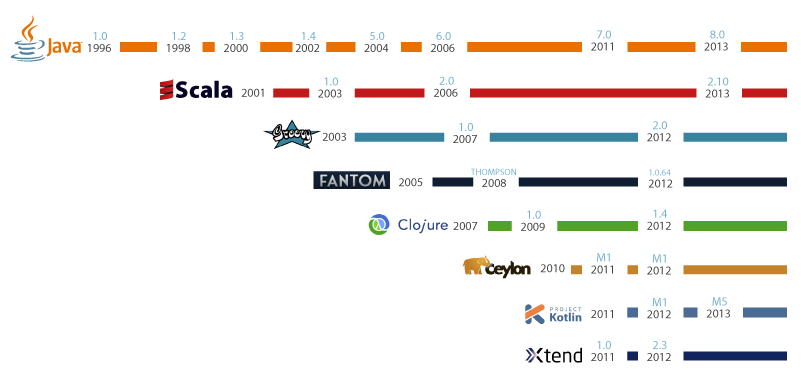
\includegraphics[width=\linewidth]{Images/jvm-languages}
	\end{figure}
\end{frame}

\begin{frame}{Lenguaje}
	\begin{figure}
		\centering
		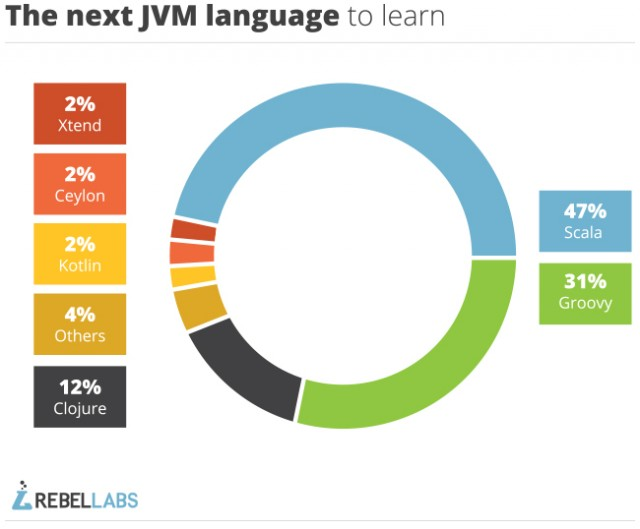
\includegraphics[width=\linewidth]{Images/next-jvm-lang}
	\end{figure}
\end{frame}

\begin{frame}{Objetivo}
	\begin{figure}
		\centering
		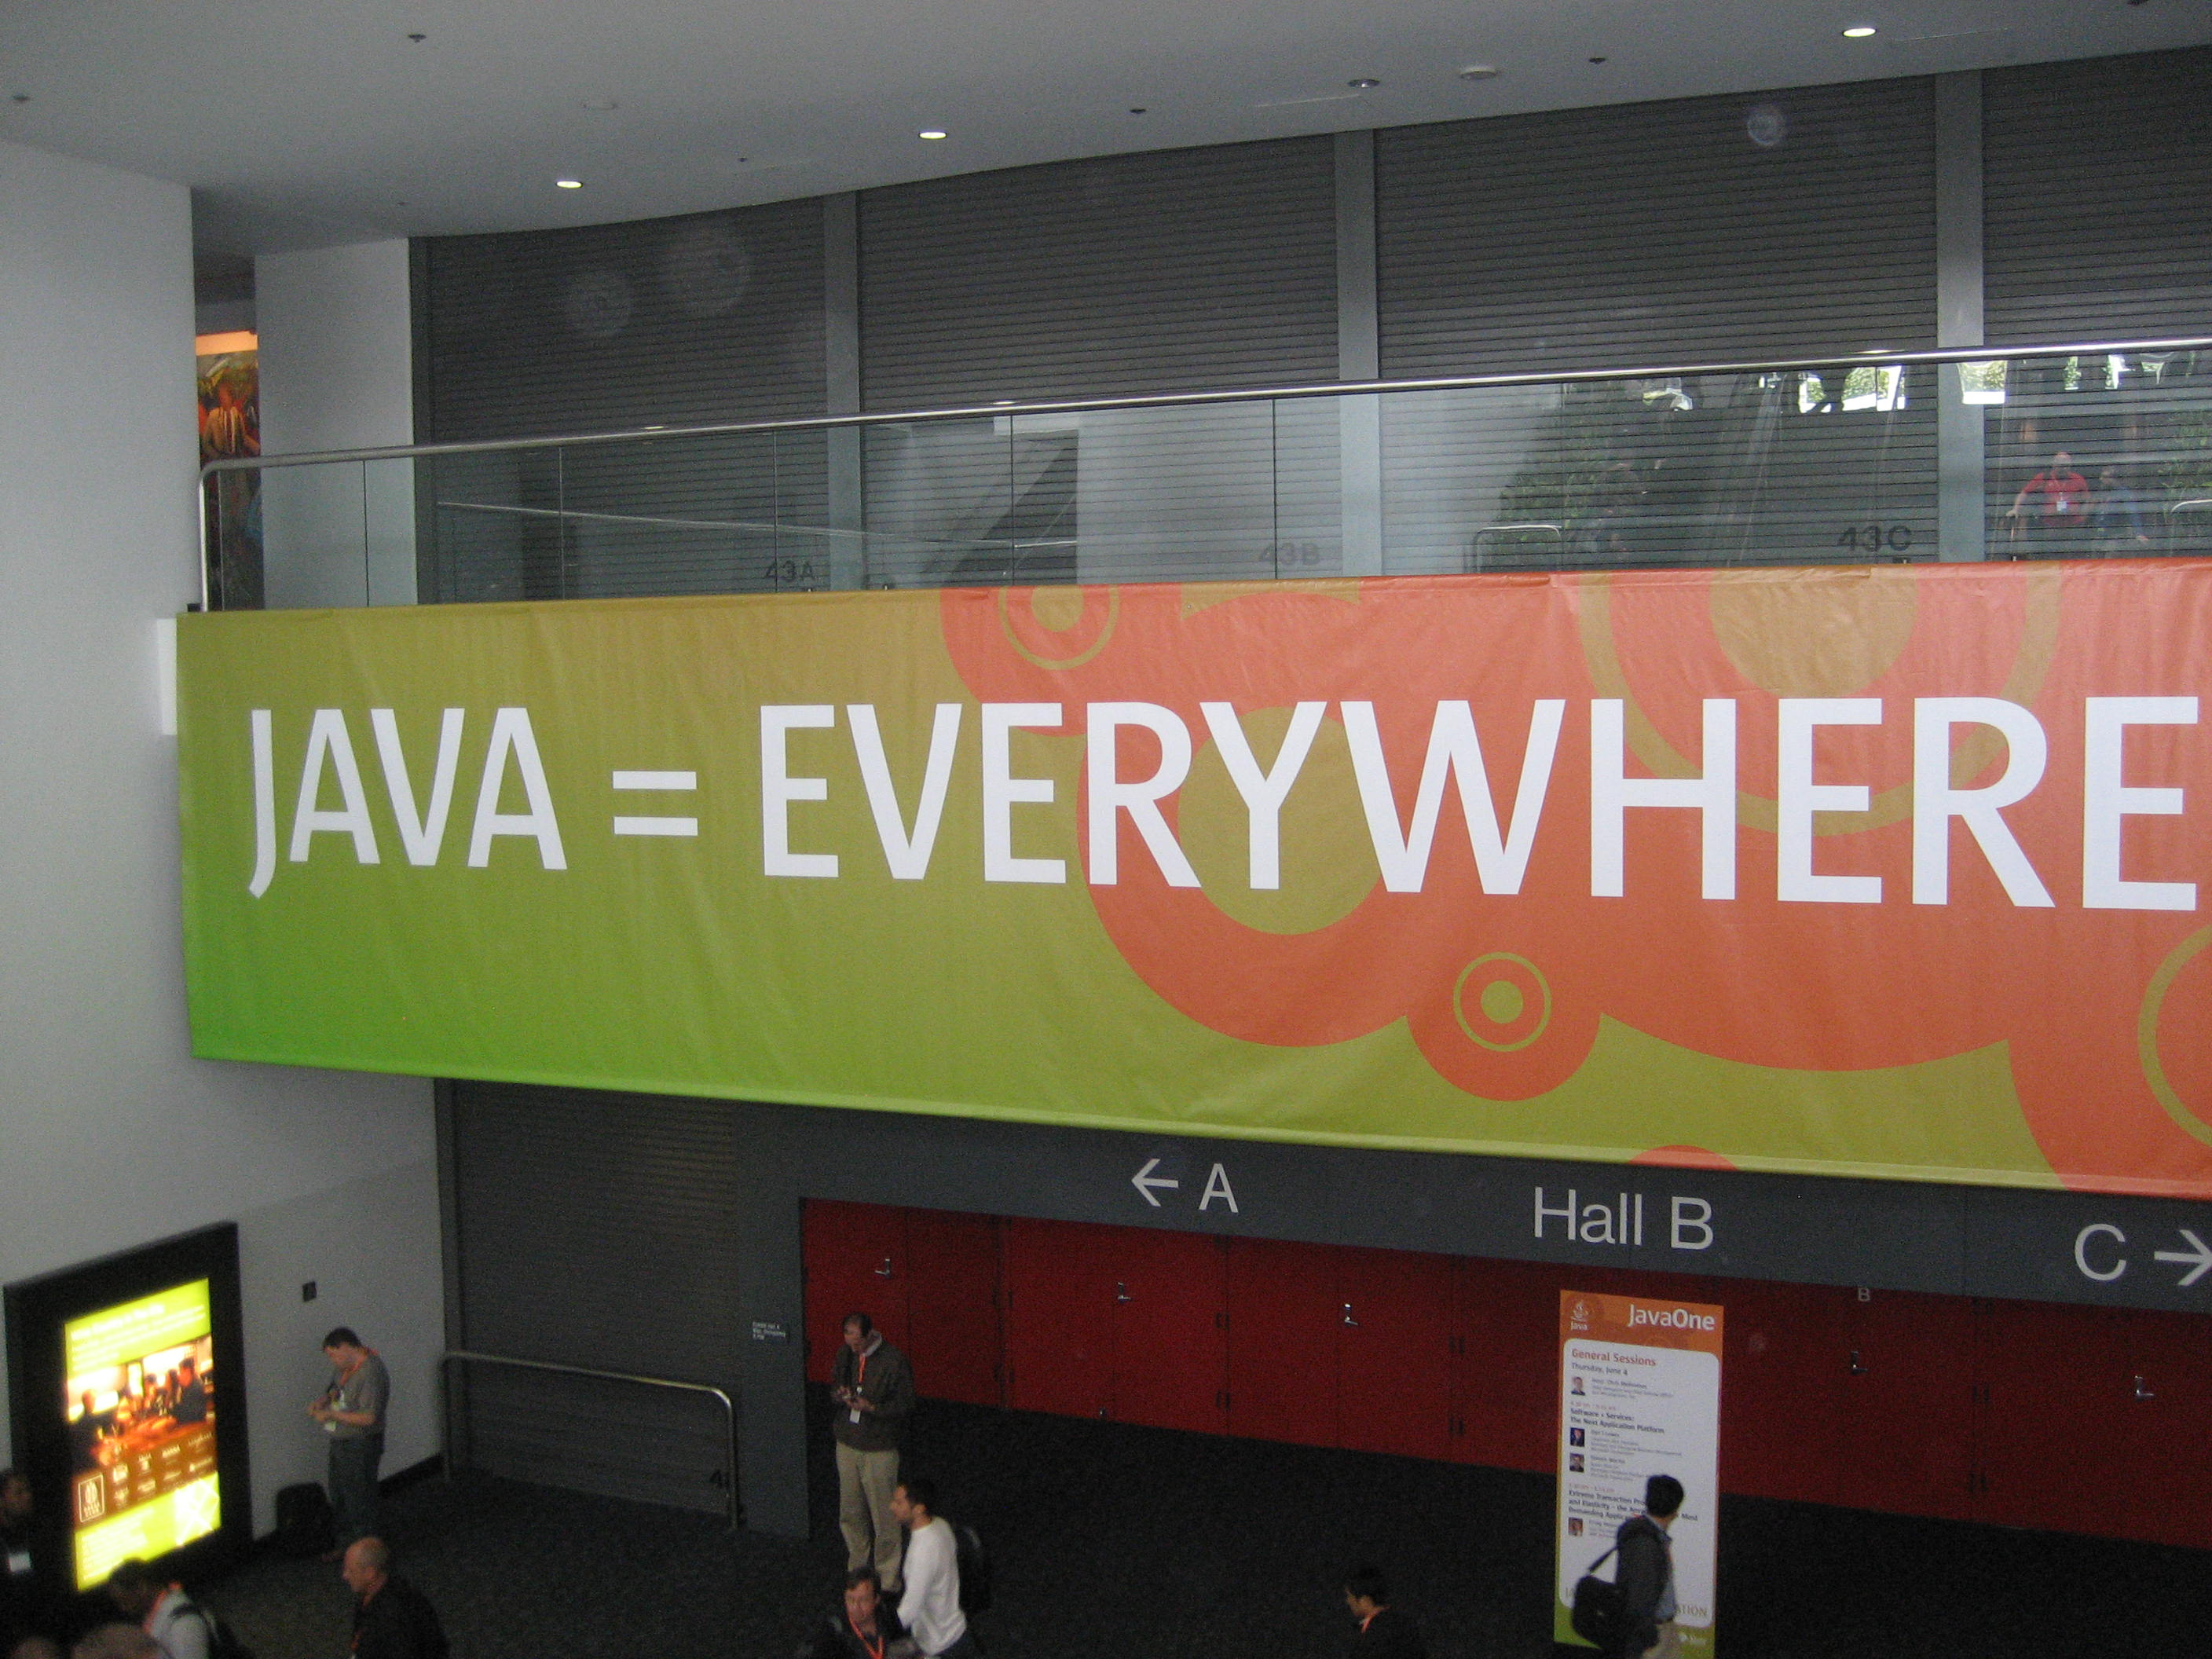
\includegraphics[width=\linewidth]{Images/everywhere}
	\end{figure}
\end{frame}

\begin{frame}{Objetivo}
	\begin{itemize}
		\item Escritorio - JSE
		\item Web/Enterprise - JEE
		\item Móvil - JME, Android
		\item Embarcado - JME
	\end{itemize}
\end{frame}

\begin{frame}{Maquina}
	\begin{figure}
		\centering
		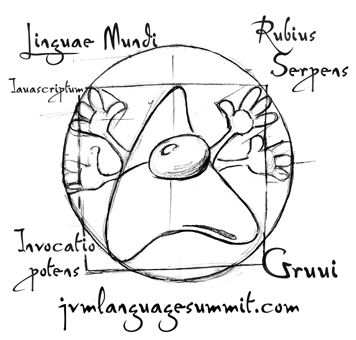
\includegraphics[width=0.7\linewidth]{Images/DukeVitru}
	\end{figure}
\end{frame}

\begin{frame}{Maquina}
	\begin{itemize}
		\item HotSpot(Oracle)
		\item OpenJDK(Oracle, Red Hat, IBM)
		\item IcedTea (Red Hat)
		\item IBM J9
		\item Zulu (Azul)
		\item Zing (Azul)
		\item Java HP-UX
		\item Excelsior JET
	\end{itemize}
\end{frame}

\begin{frame}{Framework}
	\begin{figure}
		\centering
		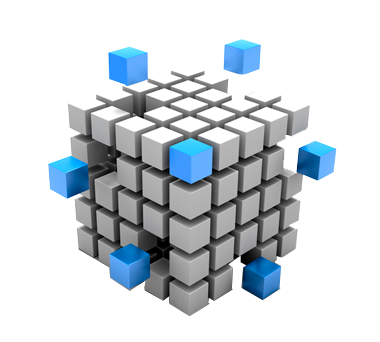
\includegraphics[width=0.7\linewidth]{Images/framework}
	\end{figure}
\end{frame}

\begin{frame}{Framework - Web}
	\begin{figure}
		\centering
		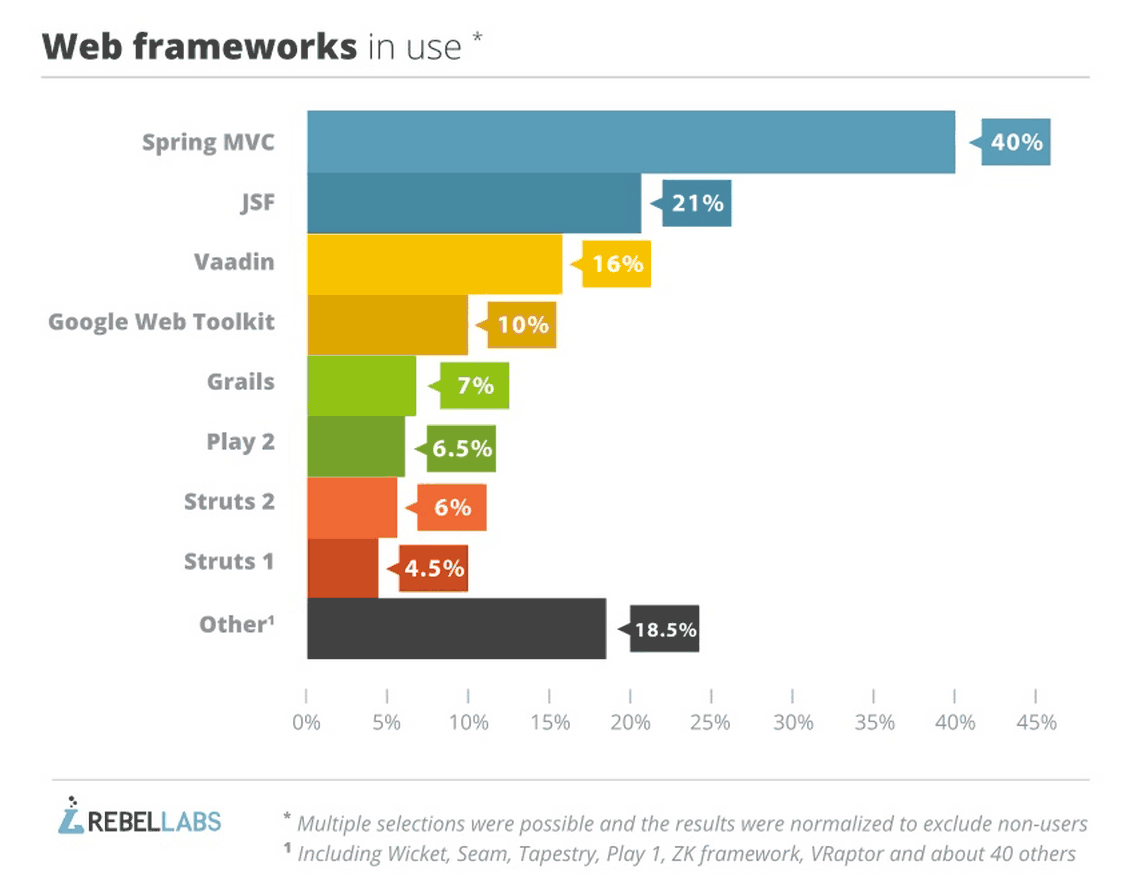
\includegraphics[width=0.9\linewidth]{Images/fwweb}
	\end{figure}
\end{frame}

\begin{frame}{Framework - Enterprise}
	\begin{figure}
		\centering
		
\includegraphics[width=\linewidth]{Images/javaeesp}
	\end{figure}
\end{frame}

\begin{frame}{Framework - Ligero}
	\begin{figure}
		\centering
		
\includegraphics[width=0.9\linewidth]{Images/ecosystem}
	\end{figure}
\end{frame}

\begin{frame}{Framework - Embarcado}
	\begin{figure}
		\centering
		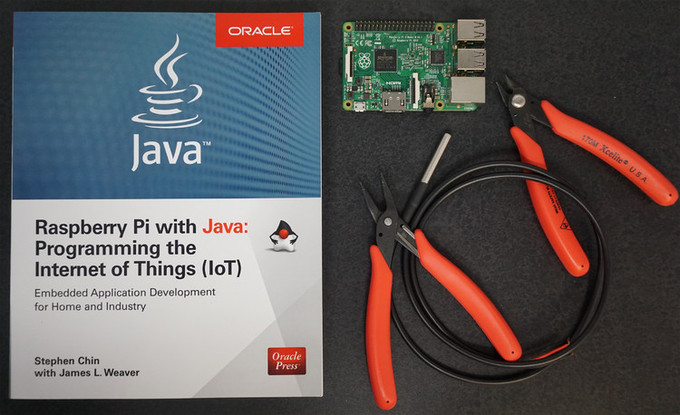
\includegraphics[width=0.9\linewidth]{Images/javapy}
	\end{figure}
\end{frame}

\begin{frame}{Framework - Movil}
	\begin{figure}
		\centering
		
\includegraphics[width=0.9\linewidth]{Images/android}
	\end{figure}
\end{frame}



\begin{frame}{Herramientas}
	\begin{figure}
		\centering
		
\includegraphics[width=0.5\linewidth]{Images/bob}
	\end{figure}
\end{frame}

\begin{frame}{Herramientas}
	\begin{figure}
		\centering
		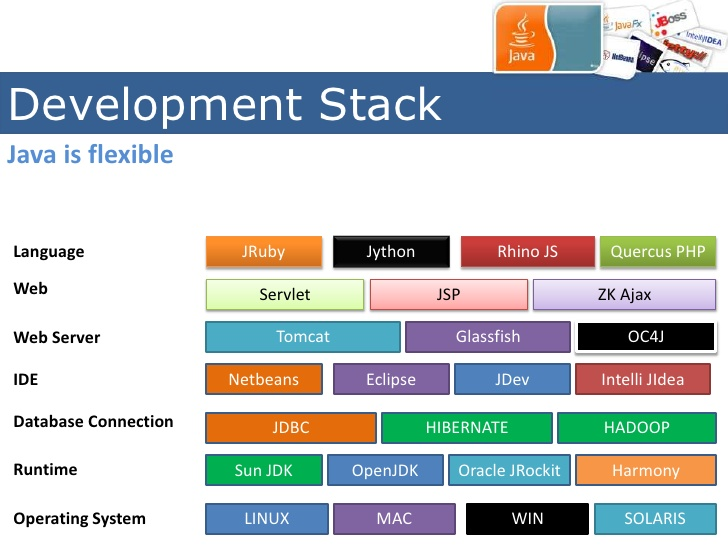
\includegraphics[width=0.9\linewidth]{Images/flexible}
	\end{figure}
\end{frame}

\begin{frame}{Herramientas}
	\begin{figure}
		\centering
		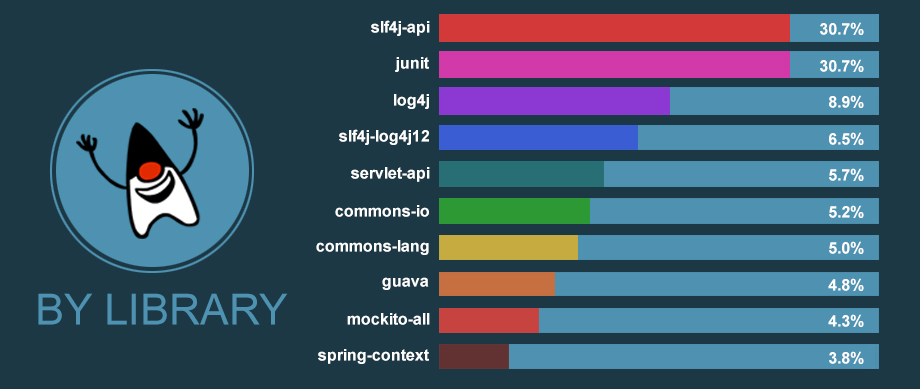
\includegraphics[width=0.9\linewidth]{Images/library}
	\end{figure}
\end{frame}


\begin{frame}{Herramientas}
	\begin{figure}
		\centering
		
\includegraphics[width=0.9\linewidth]{Images/ide}
	\end{figure}
\end{frame}


\begin{frame}{Lecturas adicionales}
	\begin{itemize}
		\item \href{http://zeroturnaround.com/rebellabs/java-tools-and-technologies-landscape-for-2014/}{Java Landscape Report - RebelLabs}
		\item\href{http://www.oracle.com/technetwork/topics/newtojava/intro-142494.html}{Java Technology concept map}
	\end{itemize}
\end{frame}


\section{Fin}

\begin{frame}{Gracias}
\begin{itemize}
\item me@vorozco.com
\item http://vorozco.com
\item http://github.com/tuxtor/slides
\end{itemize}
\begin{center}

\includegraphics[width=0.1\linewidth]{Images/cclogo}
\\
This work is licensed under a Creative Commons Attribution-ShareAlike 3.0 Guatemala License.
\end{center}
\end{frame}
\end{document}

